\documentclass[11pt]{article}
\usepackage[margin=1in]{geometry}
\usepackage{graphicx}
\usepackage{booktabs}
\usepackage{float}
\usepackage{parskip}
\renewcommand{\familydefault}{\rmdefault}

\title{Yellow Pages Data: Supplementary Visualizations}
\author{For Review}
\date{\today}

\begin{document}
\maketitle

This document presents six visualizations constructed from the Yellow Pages / Dun \& Bradstreet phonebook data. Each figure is accompanied by a description of its construction and motivation.

%% ============================================================
\section*{1. Card Plan Market Shares}

\begin{center}
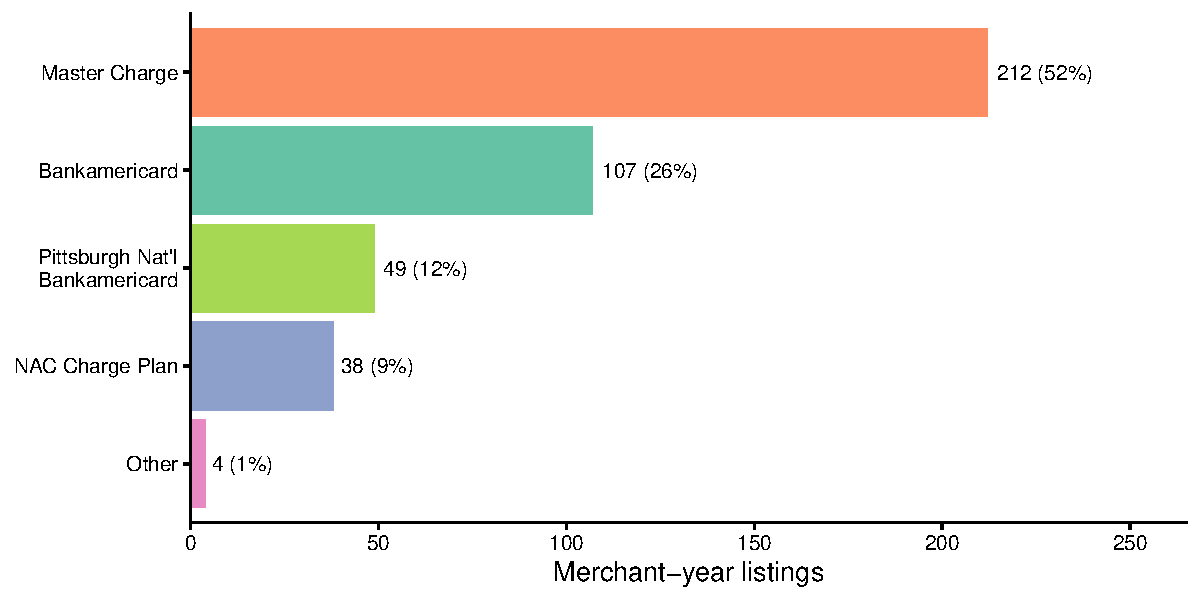
\includegraphics[width=0.85\textwidth]{1_plan_shares.pdf}
\end{center}

\textbf{Construction.} From the 410 merchant-year observations in \texttt{db\_phonebooks\_merged.csv} where \texttt{offers\_credit} is non-zero, I tabulate the credit card plan affiliation recorded in the \texttt{phonebook\_credit\_plan} field. Plans are grouped into four categories: Master Charge (including ``Master Charge-Bank Charge Plan''), Bankamericard (excluding the Pittsburgh National variant), Pittsburgh National Bankamericard, and NAC Charge Plan. Bell System Credit Cards (4 observations) are grouped into ``Other.''

\textbf{Motivation.} This figure documents the competitive landscape of bank card networks in the early 1970s. Master Charge (later MasterCard) held a 51\% share among accepting merchants, roughly double Bankamericard (later Visa) at 26\%. The Pittsburgh National Bankamericard variant (12\%) reflects local bank issuance under the Bankamericard umbrella. The NAC Charge Plan (9\%) was a regional network. This composition is informative about network competition in the early period and the degree of local vs.\ national network penetration.

\newpage

%% ============================================================
\section*{2. Credit Card Introduction Map}

\begin{center}
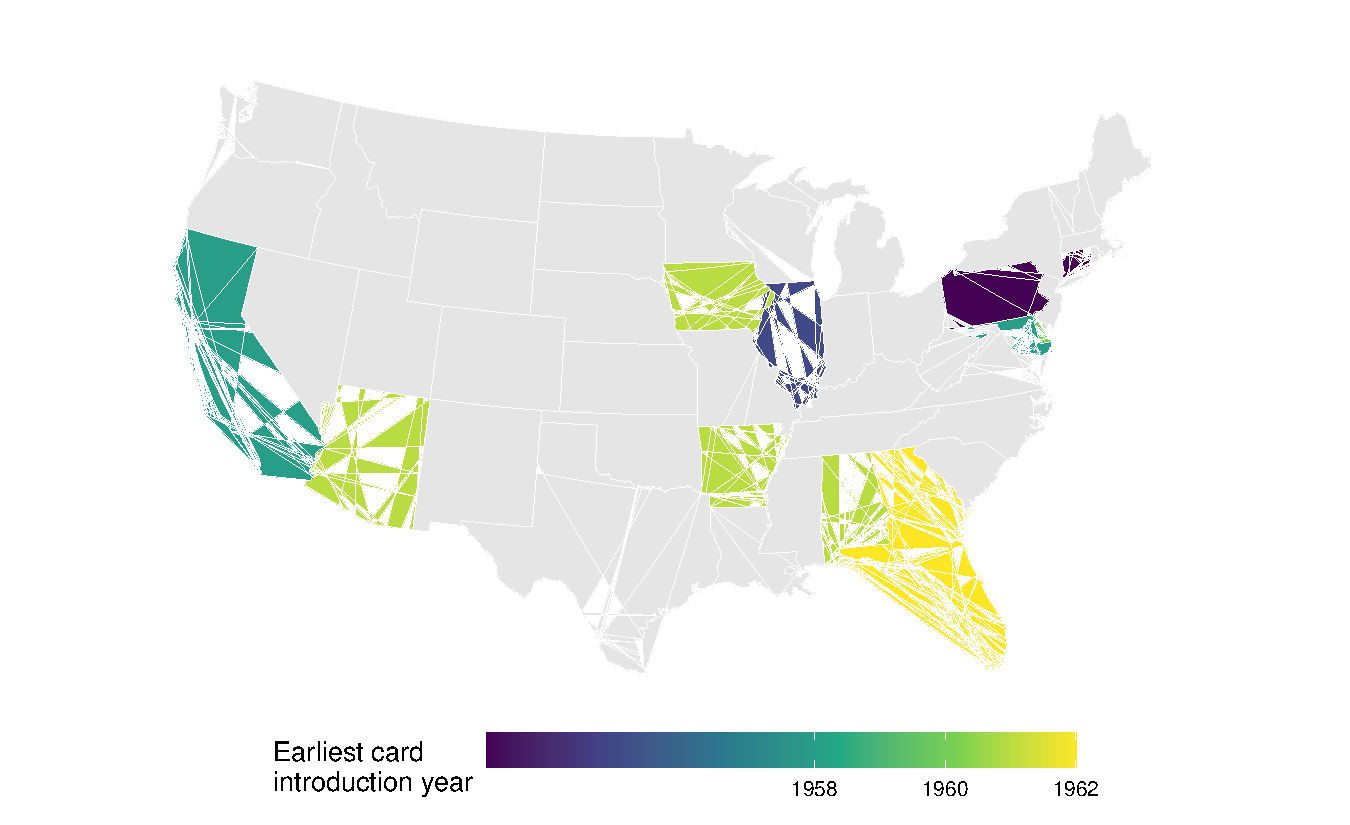
\includegraphics[width=0.85\textwidth]{2_intro_map.pdf}
\end{center}

\textbf{Construction.} From \texttt{Introduction Dates.xlsx}, which records the earliest observed credit card listing in each Yellow Pages phonebook by geography, I extract the four-digit year from the \texttt{Card\_intro} field (which uses ``+'' and ``-'' suffixes for bounds). I aggregate to the state level by taking the minimum introduction year across all cities in each state, then merge with the built-in US state map via \texttt{maps::map\_data("state")}.

\textbf{Motivation.} This map shows the geographic diffusion of bank credit card networks across the United States. States with the earliest introduction dates (California, where BankAmericard originated in 1958) are visually distinguished from states where cards arrived later. The map helps assess whether the geographic pattern of card availability is related to the usury treatment assignment used in the identification strategy. States without phonebook coverage in the Library of Congress collection appear in grey.

\newpage

%% ============================================================
\section*{3. Phonebook Coverage Over Time by State}

\begin{center}
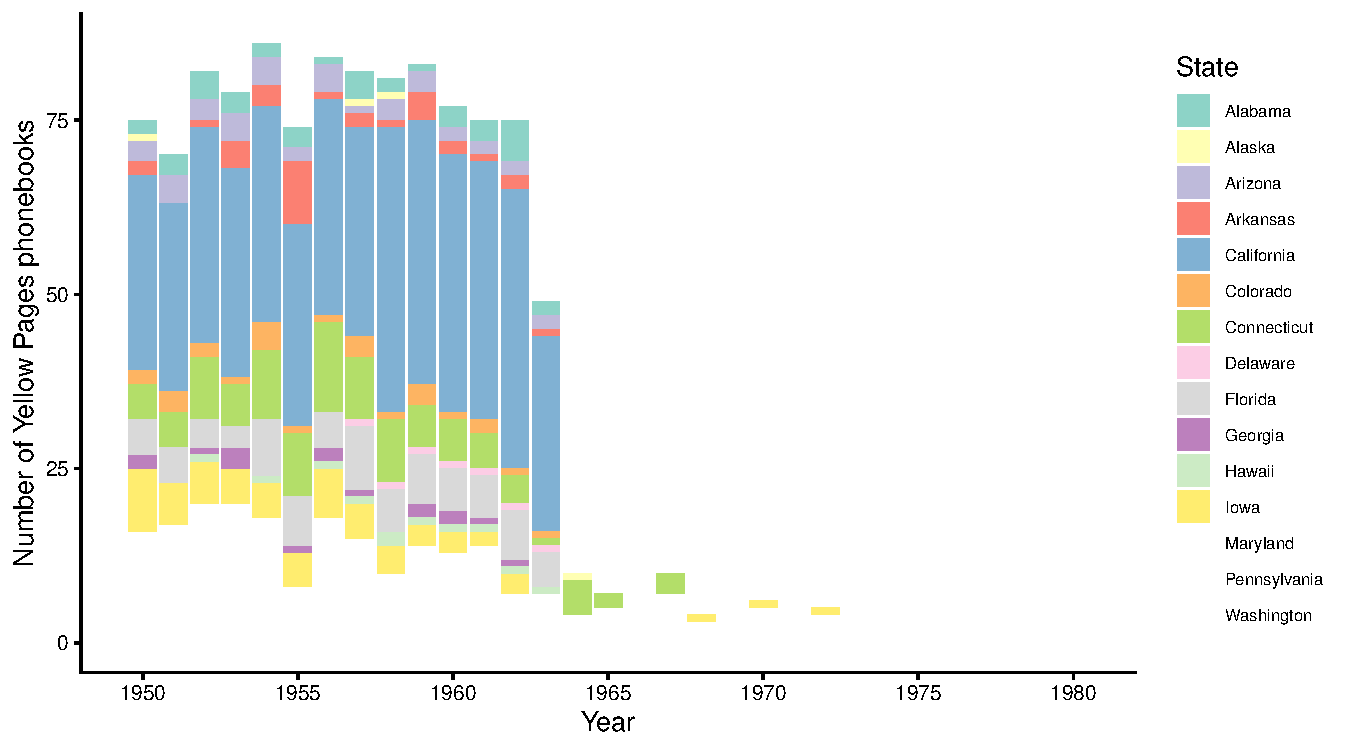
\includegraphics[width=0.85\textwidth]{3_coverage_by_state.pdf}
\end{center}

\textbf{Construction.} From \texttt{pages\_include\_pagenumbers.csv}, I filter to included Yellow Pages phonebooks (\texttt{include == 1}, \texttt{yellow == 1}) and extract the state name from the Library of Congress title field. I count the number of phonebooks available per year and state for the period 1950--1980.

\textbf{Motivation.} This figure documents the scope of the Library of Congress US Telephone Directory collection that underlies the data collection effort. The stacked bar chart shows how phonebook availability varies across years and states. Coverage peaks in the early-to-mid 1960s and declines in later years, reflecting the Library of Congress's digitization priorities. The state composition reveals which geographic areas contribute the most phonebook-years to the analysis, relevant for assessing external validity and potential geographic selection.

\newpage

%% ============================================================
\section*{4. Acceptance by Industry and Firm Size}

\begin{center}
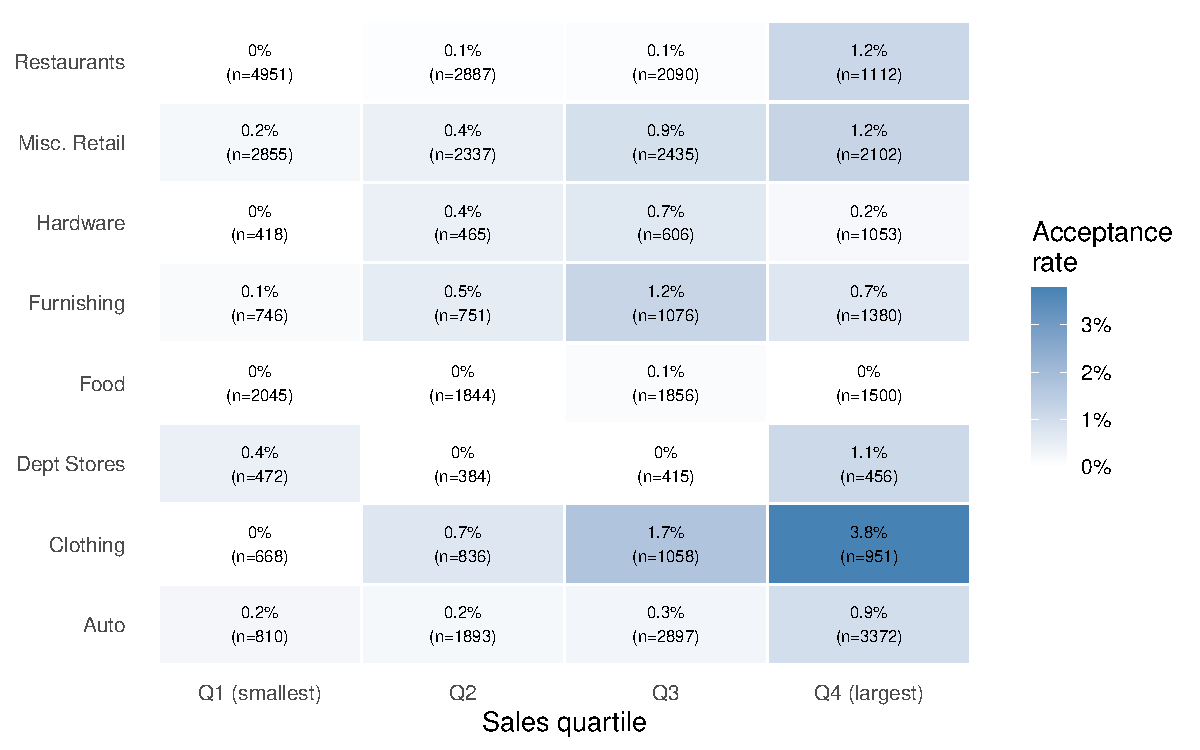
\includegraphics[width=0.85\textwidth]{4_acceptance_heatmap.pdf}
\end{center}

\textbf{Construction.} From the subset of \texttt{db\_phonebooks\_merged.csv} firms located in phonebook-covered areas (\texttt{covered\_by\_phonebooks} $\neq$ 0) with positive sales data, I assign each firm to a 2-digit SIC industry and a sales quartile (computed across all retail firms with sales data). I then compute the card acceptance rate (fraction with \texttt{offers\_credit} $\neq$ 0) within each industry $\times$ size quartile cell. Cells with fewer than 10 observations are excluded.

\textbf{Motivation.} This figure examines two dimensions of card adoption heterogeneity simultaneously. The adoption regression (Table 2 in the paper) shows that larger firms and single-establishment firms are more likely to accept cards. This heat map provides a non-parametric view of the same relationship, revealing whether the size gradient varies across industries. The pattern is informative about whether cost reduction (which predicts adoption by undiversified, high-volume firms) or demand-steering (which predicts adoption by low-share firms) dominates.

\newpage

%% ============================================================
\section*{5. Phonebook Size Trends}

\begin{center}
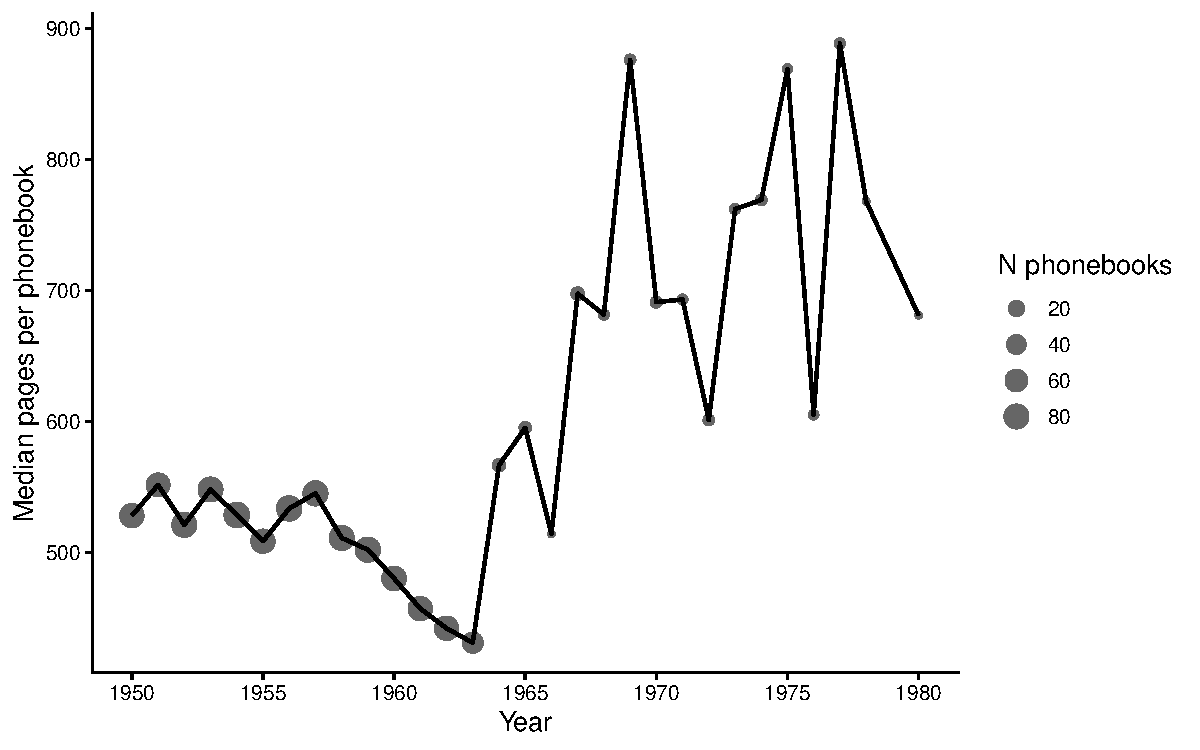
\includegraphics[width=0.85\textwidth]{5_phonebook_size.pdf}
\end{center}

\textbf{Construction.} From \texttt{pages\_include\_pagenumbers.csv}, using included Yellow Pages phonebooks from 1950--1980, I compute the median page count per year. Point sizes are proportional to the number of phonebooks available in each year.

\textbf{Motivation.} Phonebook page counts serve as a proxy for the breadth of commercial activity in a market. Growing phonebooks may reflect expanding Yellow Pages advertising, more business categories, or growing local economies. This figure provides context for the data collection: larger phonebooks are more likely to have dedicated ``Credit Card'' sections, so the trend in phonebook size may affect the probability of observing card acceptance listings. A secular increase in phonebook size would be consistent with urbanization and commercial growth, while a flat or declining trend might suggest digitization selection effects in the Library of Congress collection.

\newpage

%% ============================================================
\section*{6. Geographic Concentration of Early Adopters}

\begin{center}
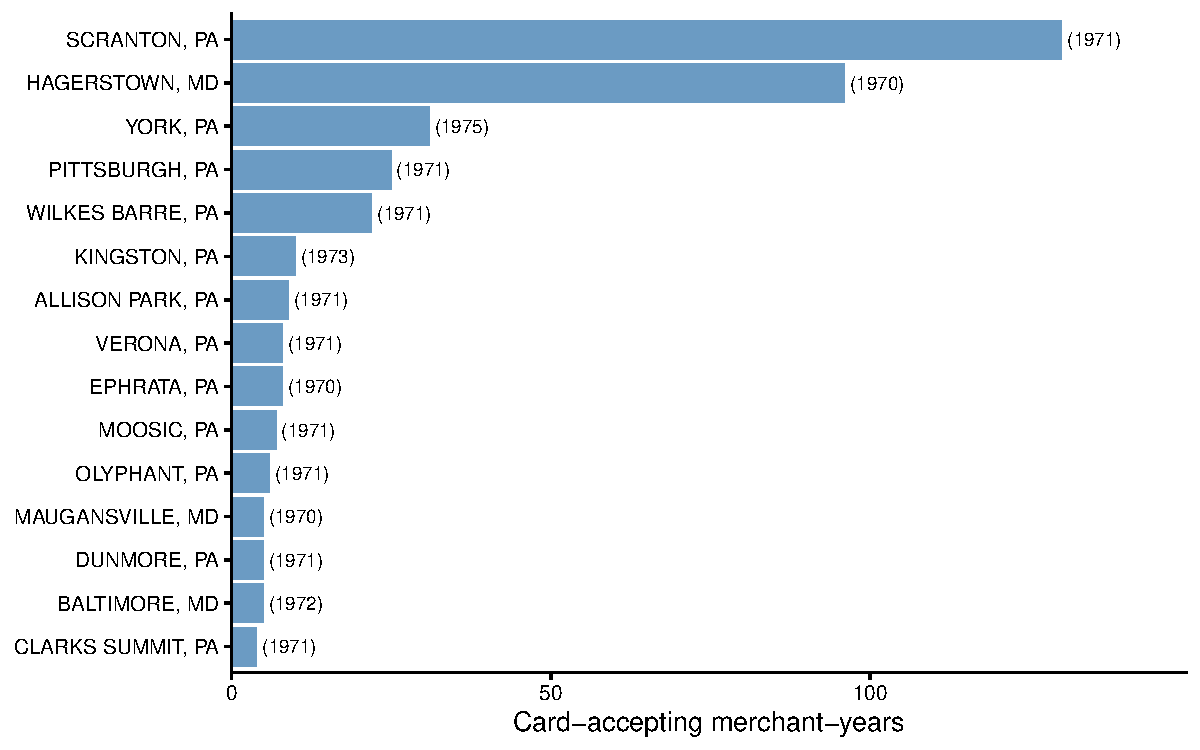
\includegraphics[width=0.85\textwidth]{6_geographic_concentration.pdf}
\end{center}

\textbf{Construction.} From the card-accepting merchant-years in \texttt{db\_phonebooks\_merged.csv}, I count the number of accepting merchant-year observations by city and state, and record the first year of card acceptance in each city. The top 15 cities by total merchant-year count are plotted, with the year of first observed acceptance annotated in parentheses.

\textbf{Motivation.} This figure reveals where the card acceptance data is geographically concentrated. Scranton, PA dominates with 130 merchant-years (reflecting the city's early and well-documented phonebook coverage), followed by Hagerstown, MD (96) and York, PA (31). The concentration in Pennsylvania and Maryland reflects both the geographic coverage of the Library of Congress phonebook collection and the early adoption patterns of bank card networks in the mid-Atlantic region. The year annotations show that most cities' first observed acceptance dates cluster in the early 1960s, consistent with the national rollout of BankAmericard and Master Charge programs.

\newpage
\section*{Raw OCR Data: Summary}

The underlying phonebook scans were processed by Hi-Tech Inc.\ using optical character recognition (OCR). The raw OCR output --- 110 CSV files totaling approximately 1 GB --- contains word-level bounding boxes, page assignments, and automated category header detection for each phonebook. This data is available for reuse and extension.

\begin{center}
\begin{tabular}[t]{ll}
\toprule
 & \\
\midrule
Phonebooks processed (OCR) & 110\\
Total OCR words extracted & 3,745,359\\
Total pages scanned & 13,548\\
Business listings (with phone numbers) & 607,344\\
Unique business categories & 17,995\\
\addlinespace
States covered & 5\\
Cities covered & 26\\
Year range & 1950-1978\\
Median listings per phonebook & 2,052\\
Median pages per phonebook & 64\\
\addlinespace
Median categories per phonebook & 358.5\\
\bottomrule
\end{tabular}

\end{center}

The OCR pipeline extracted 3.7 million words across 13,548 pages, identifying 607,344 business listings (defined as entries containing phone numbers) and 17,995 unique Yellow Pages category headers. The ``Credit Card \& Other Credit Plans'' category --- from which the 510 card-accepting merchant-years were manually transcribed --- appears in 11 of the 110 phonebooks.

%% ============================================================
\newpage
\section*{7. OCR-Processed Phonebooks by State and Year}

\begin{center}
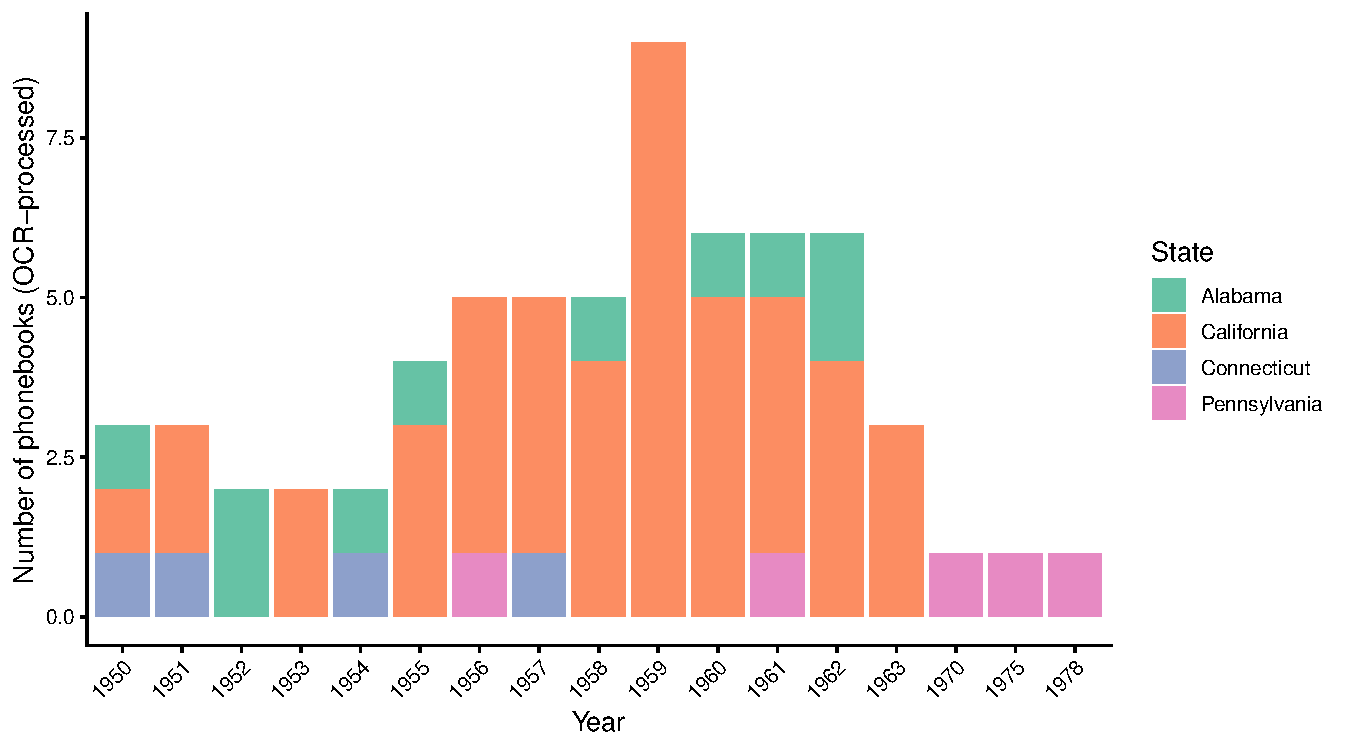
\includegraphics[width=0.85\textwidth]{7_ocr_books_by_year.pdf}
\end{center}

\textbf{Construction.} From the 110 OCR-processed CSV files, I extract the state and year metadata from each file. Each bar represents one year; colors indicate the state of origin.

\textbf{Motivation.} This figure documents the temporal and geographic scope of the raw OCR data that underlies the credit card acceptance data collection. The OCR processing covers phonebooks from 1950 to 1978, concentrated in Pennsylvania and California. The distribution reveals the sampling frame: phonebooks were selected from the Library of Congress collection based on geographic coverage of the Dun \& Bradstreet business panel, with priority given to states with both treated and control usury regimes.

%% ============================================================
\newpage
\section*{8. Business Listings per Phonebook}

\begin{center}
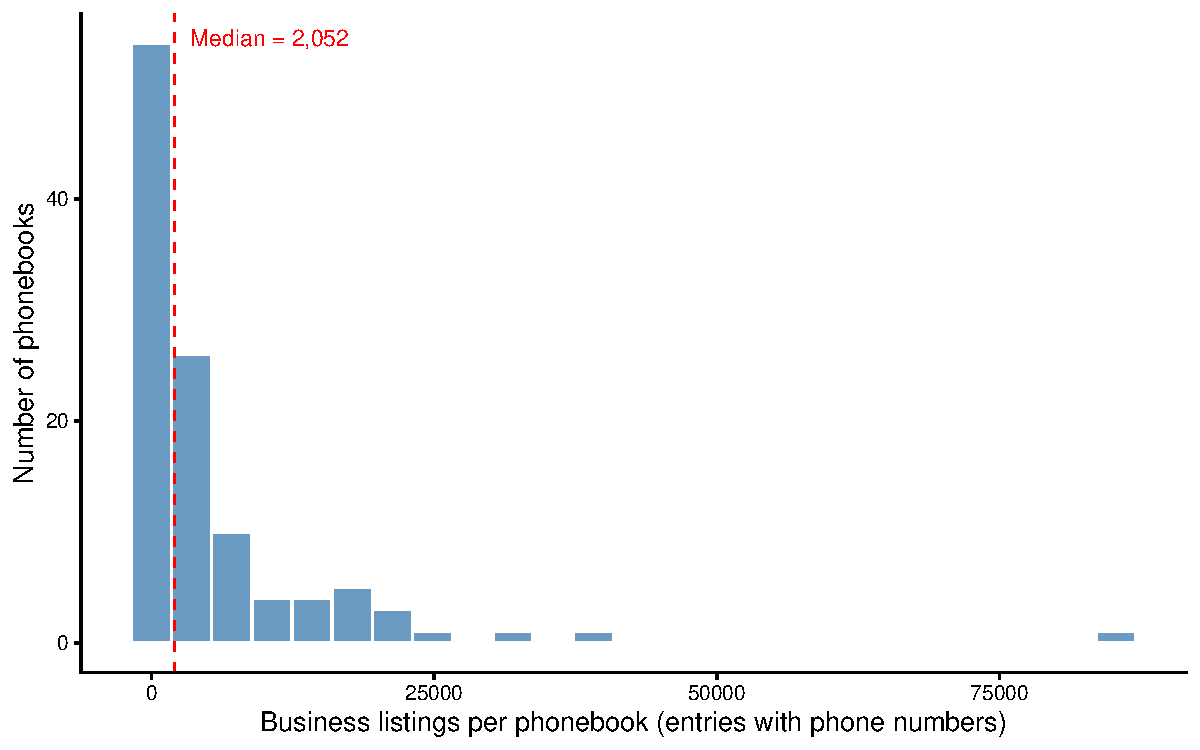
\includegraphics[width=0.85\textwidth]{8_listings_per_book.pdf}
\end{center}

\textbf{Construction.} For each of the 110 OCR-processed phonebooks, I count the number of text entries that contain a phone number (\texttt{has.number == 1}), which proxies for individual business listings. The dashed red line marks the median.

\textbf{Motivation.} The distribution of listings per phonebook characterizes the density of commercial activity captured by the data. The median phonebook contains approximately 2,000 business listings. Larger phonebooks (up to 30,000+ listings) correspond to major metropolitan areas. This figure helps assess the representativeness of the sample: phonebooks with more listings provide denser local coverage of the business population.

%% ============================================================
\newpage
\section*{9. Most Common Yellow Pages Categories}

\begin{center}
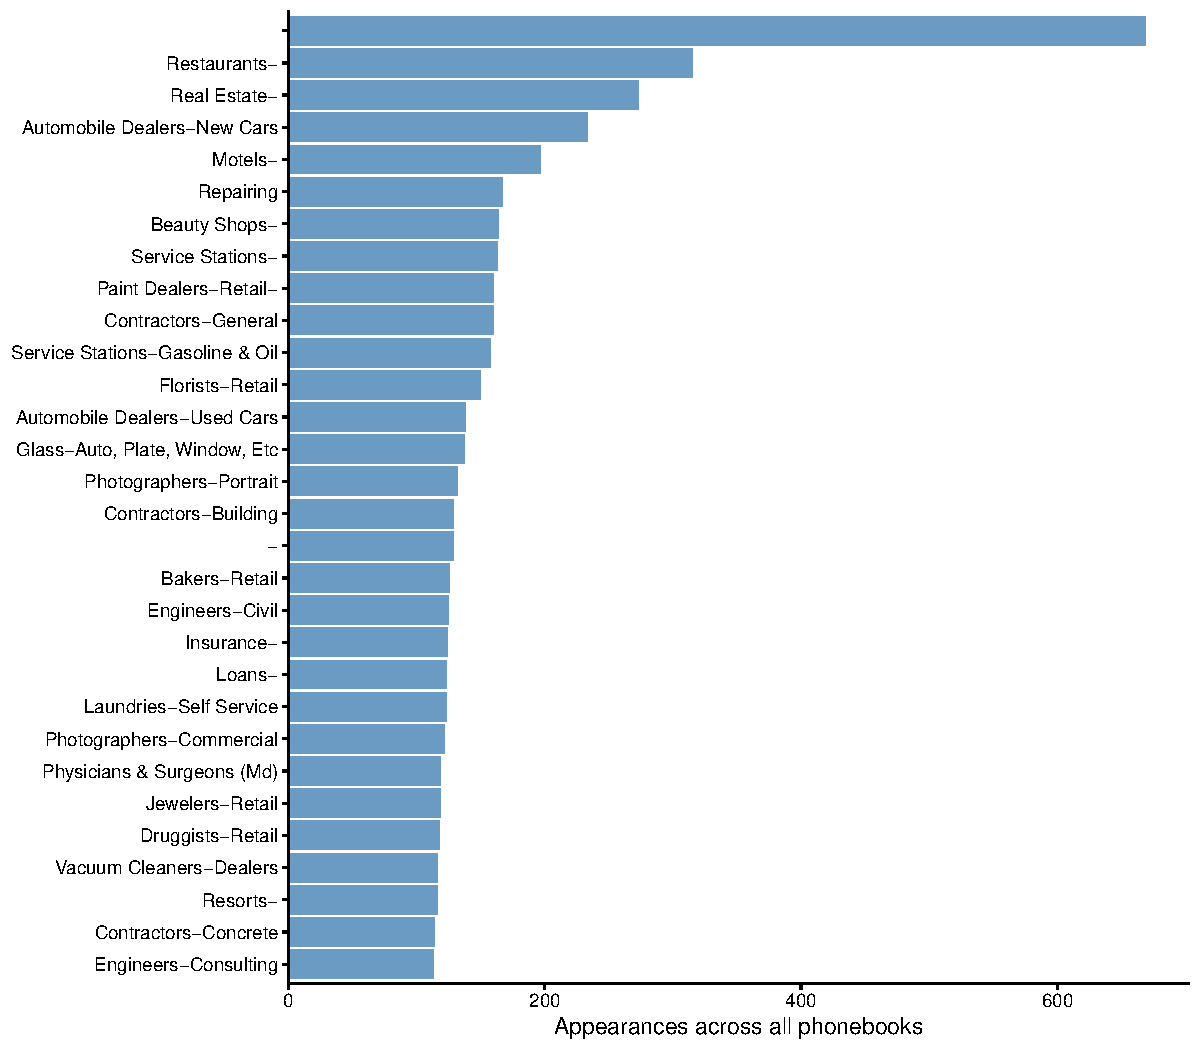
\includegraphics[width=0.85\textwidth]{9_top_categories.pdf}
\end{center}

\textbf{Construction.} From all 110 phonebooks, I extract text entries flagged as category headers (\texttt{is\_title == 1}) and clean the category names (removing ``Cont'd'' suffixes and standardizing capitalization). I count the number of phonebooks in which each category appears and plot the top 30.

\textbf{Motivation.} The Yellow Pages category structure reveals the organization of local commercial directories in mid-20th century America. The most common categories --- automobile dealers, insurance, contractors, plumbers --- reflect the service-oriented nature of local business directories. Notably, ``Credit Card \& Other Credit Plans'' is a distinct category that appears in 11 phonebooks, confirming that credit card acceptance was treated as a standalone directory section rather than being embedded within individual business listings.

%% ============================================================
\newpage
\section*{10. Pages per Phonebook Over Time}

\begin{center}
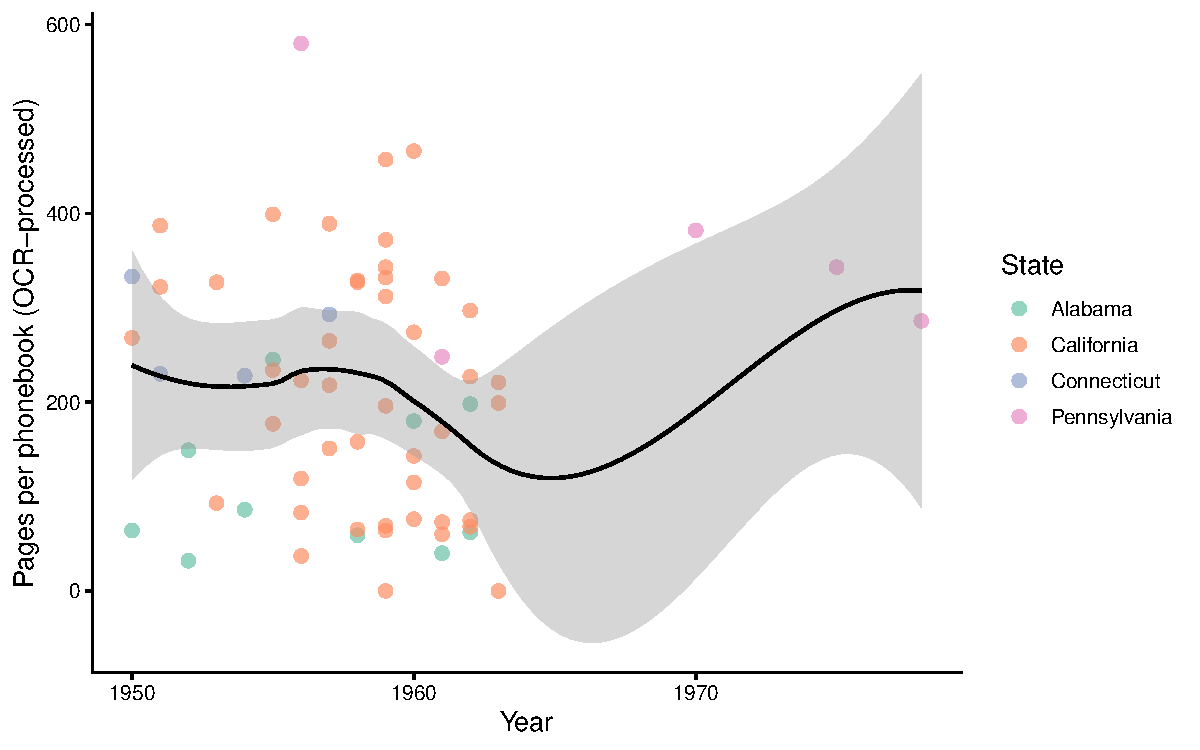
\includegraphics[width=0.85\textwidth]{10_pages_over_time.pdf}
\end{center}

\textbf{Construction.} For each OCR-processed phonebook, I count the number of unique pages and plot against the phonebook year. Points are colored by state; a LOESS smoother shows the overall trend.

\textbf{Motivation.} Phonebook size (measured in pages) serves as a proxy for market size and commercial density. The upward trend through the 1960s and 1970s is consistent with growing commercial activity and expanding Yellow Pages advertising. Pennsylvania phonebooks (green) span the full time range, while California phonebooks (grey) are concentrated in the 1950s--1960s. The variation in size helps contextualize the data collection: larger phonebooks are more likely to contain dedicated ``Credit Card'' sections.

%% ============================================================
\newpage
\section*{11. Credit-Related Category Entries Over Time}

\begin{center}
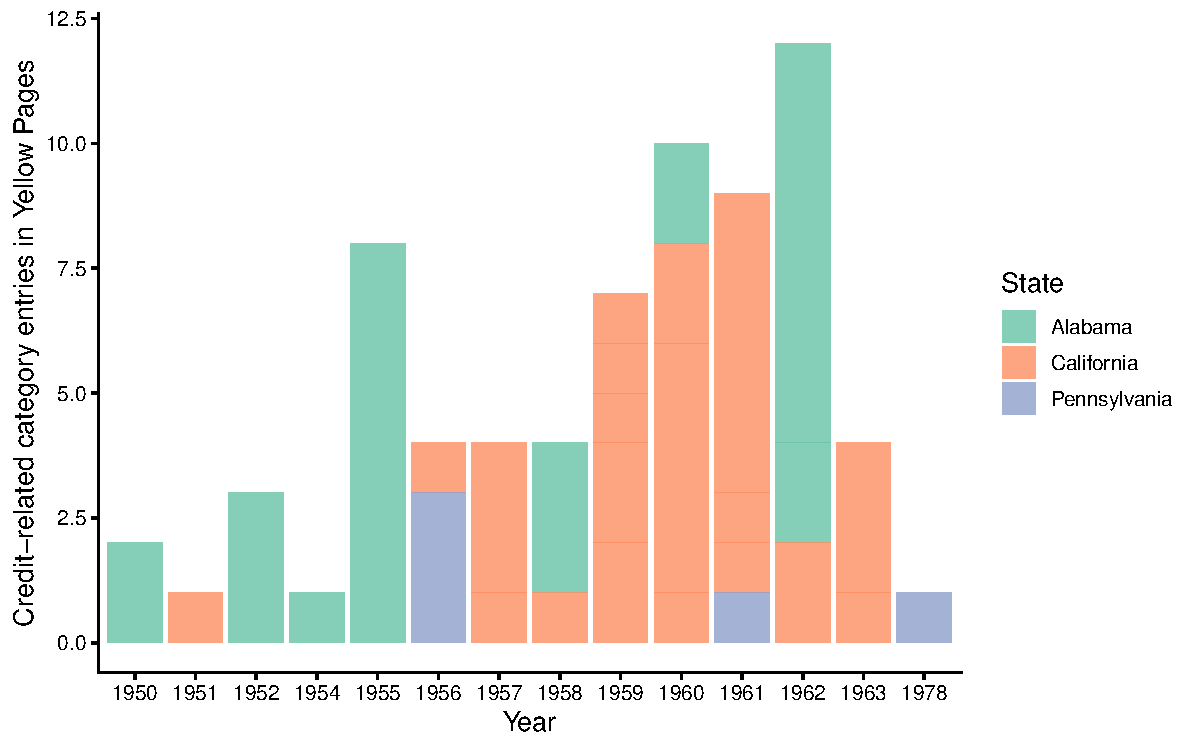
\includegraphics[width=0.85\textwidth]{11_credit_categories_over_time.pdf}
\end{center}

\textbf{Construction.} I search all category headers for entries containing ``credit,'' ``charge,'' ``Bankamericard,'' ``Master Charge,'' or ``Visa'' (case-insensitive). I count the number of credit-related category entries by city, state, and year. This captures not only ``Credit Card \& Other Credit Plans'' sections but also related categories like ``Clothing-Credit,'' ``Jewelers-Credit,'' and ``Credit Reporting Agencies.''

\textbf{Motivation.} This figure traces the emergence of credit-related commercial infrastructure in the Yellow Pages over time. The appearance of dedicated credit card sections in the late 1960s and early 1970s marks the transition from informal store credit to formalized bank card networks. The growth in credit-related entries reflects both the expansion of credit card programs and the increasing commercialization of credit services as a distinct business category.

%% ============================================================
\newpage
\part*{Full OCR Corpus (Merged + Page-Level)}

The raw OCR data comes in two forms: (1) 110 merged book-level CSV files produced by Hi-Tech Inc., containing word-level bounding boxes with automated category header detection (\texttt{is\_title}, \texttt{title\_corrected}); and (2) 165 page-level directories containing individual CSV files per scanned page, with raw OCR output only. After deduplication (preferring merged files where both exist), the combined corpus contains 168 phonebooks spanning 5 states, 44 cities, and the years 1950--1978.

\begin{center}
\begin{tabular}[t]{ll}
\toprule
 & \\
\midrule
Phonebooks in OCR corpus & 168\\
--- from merged book-level files & 63\\
--- from page-level files (new) & 105\\
Total pages scanned & 41,619\\
Business listings (with phone numbers) & 2,074,980\\
\addlinespace
Unique business categories & 49,447\\
Books with credit card sections & 13\\
States covered & 5\\
Cities covered & 44\\
Year range & 1950-1978\\
\bottomrule
\end{tabular}

\end{center}

The full corpus adds substantial coverage, particularly for California (106 city-year observations across dozens of cities) and fills gaps in the merged-only data. Figures A--F below characterize this expanded corpus.

%% ============================================================
\newpage
\section*{A. Full Corpus: Phonebooks by State and Year}

\begin{center}
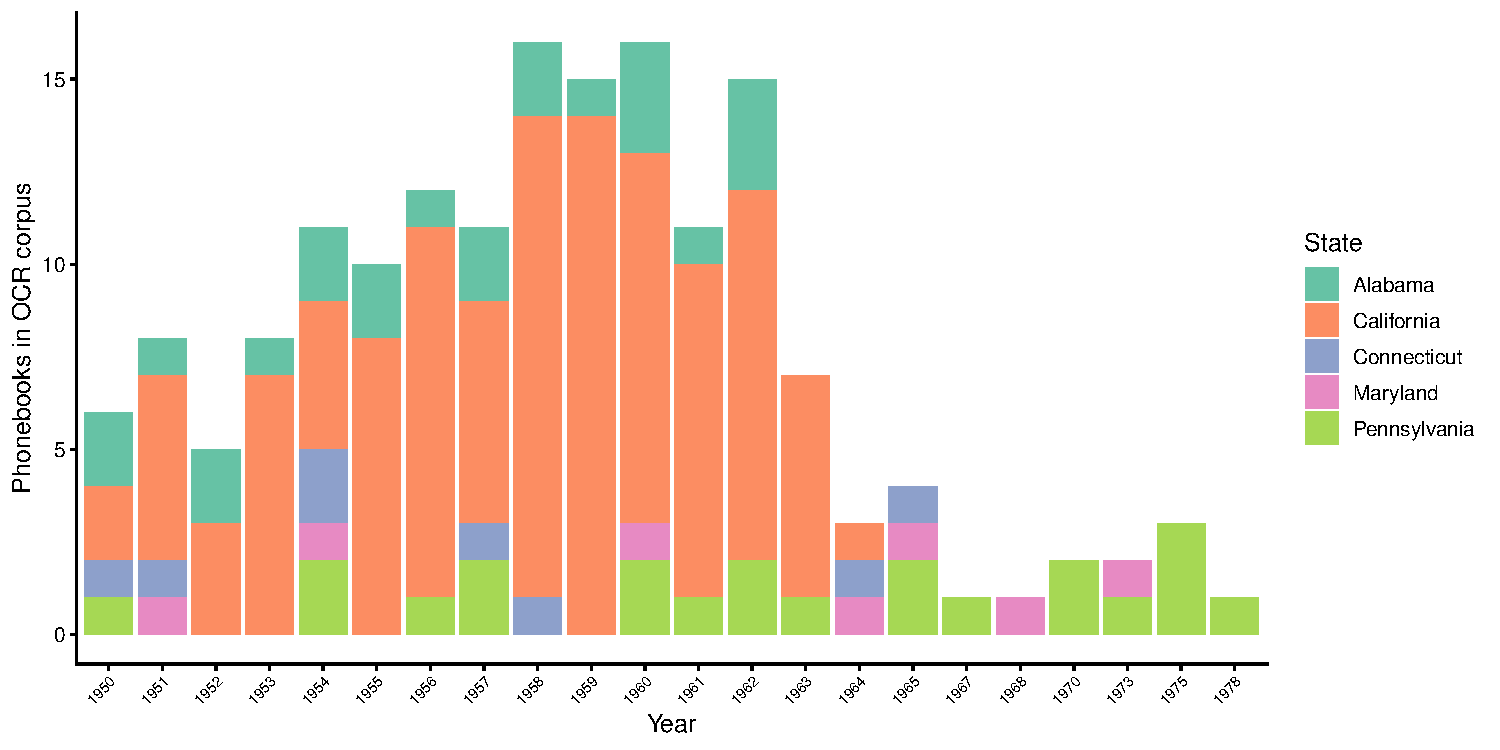
\includegraphics[width=0.85\textwidth]{A_full_corpus_by_year.pdf}
\end{center}

\textbf{Construction.} From all 168 phonebooks in the combined corpus, I count the number of phonebooks per year, colored by state. This includes both merged book-level files (63 successfully parsed) and page-level-only books (105 additional).

\textbf{Motivation.} This figure shows the dramatically expanded temporal coverage relative to the merged-only data. The addition of page-level books increases coverage in the 1950s and early 1960s, particularly for California. The expanded corpus provides a broader sampling frame for studying the pre-credit-card commercial landscape.

%% ============================================================
\newpage
\section*{B. City $\times$ Year Coverage Panel}

\begin{center}
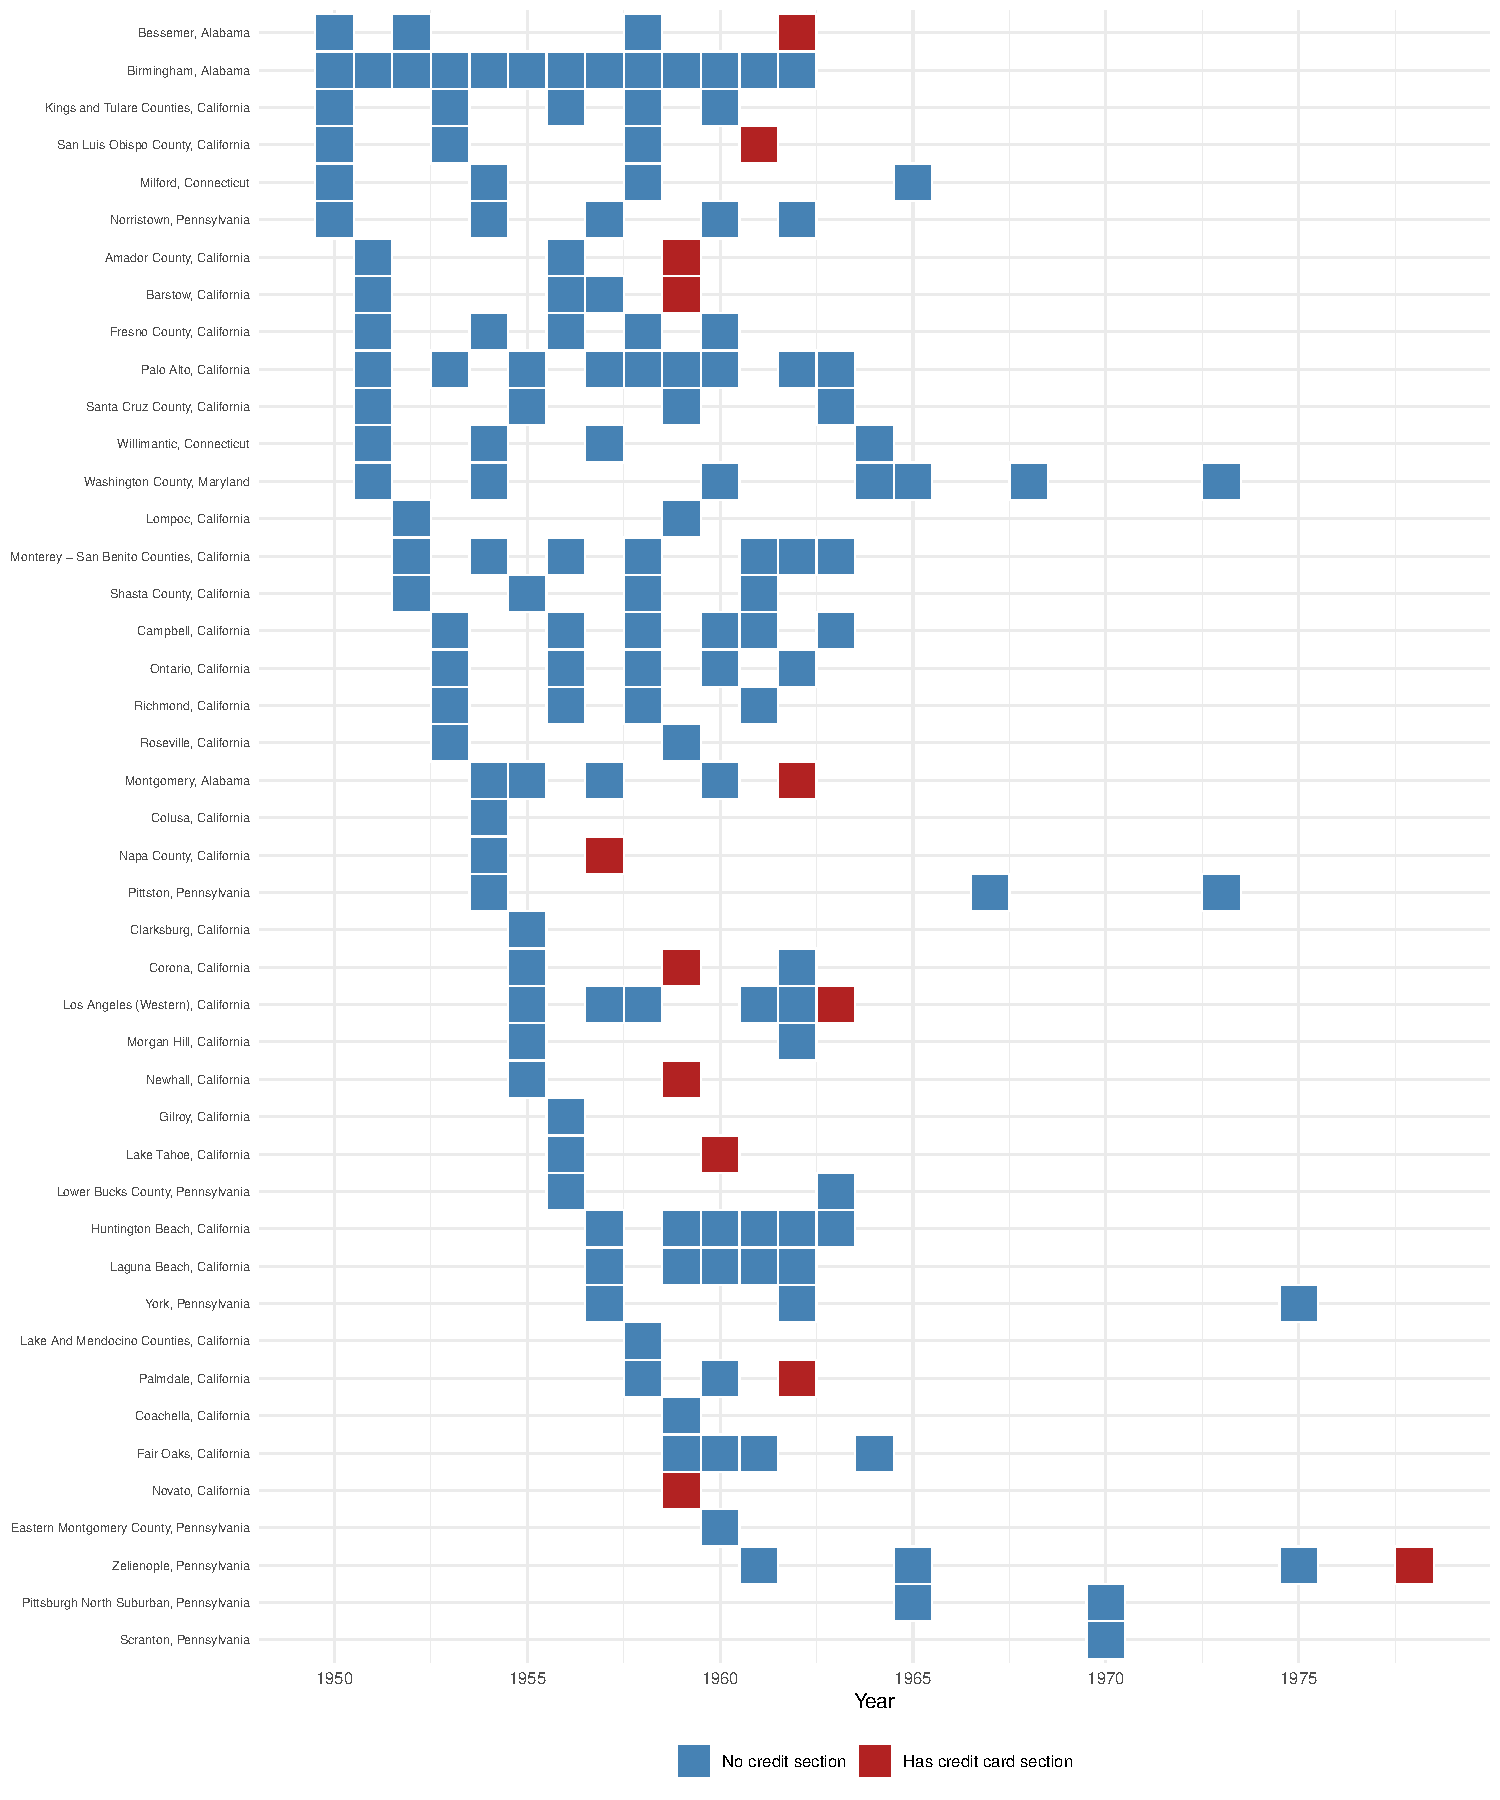
\includegraphics[width=0.85\textwidth]{B_city_year_coverage.pdf}
\end{center}

\textbf{Construction.} For each city-year pair in the corpus, I plot a tile indicating whether the phonebook has a detected credit card section (red) or not (blue). Cities are ordered by their first year of appearance. Only merged-file books have credit section detection; page-level-only books are marked as ``no credit section'' by default.

\textbf{Motivation.} This panel reveals the structure of the data: which markets are covered in which years, and where credit card sections appear. The visualization immediately shows the sparsity of coverage --- most cities have only 1--3 phonebook-years --- and highlights the geographic clustering of credit card sections in mid-Atlantic cities (Pennsylvania, Maryland) beginning in the late 1960s.

%% ============================================================
\newpage
\section*{C. California Deep Dive: BankAmericard's Home State}

\begin{center}
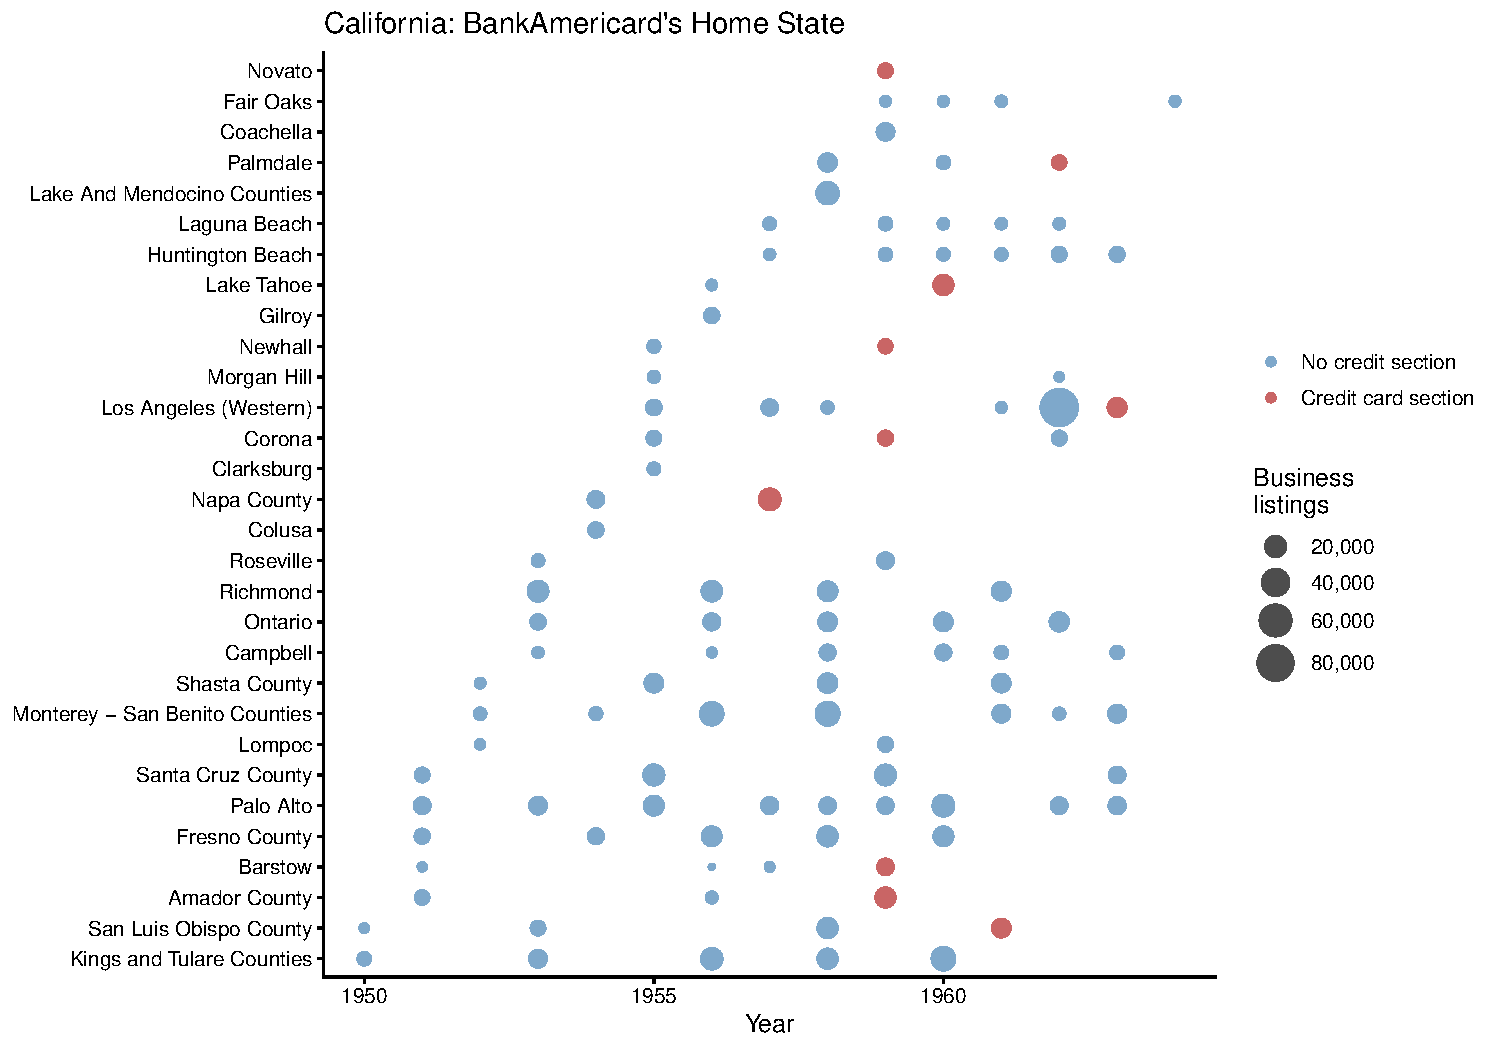
\includegraphics[width=0.85\textwidth]{C_california_deep_dive.pdf}
\end{center}

\textbf{Construction.} For California phonebooks only, I plot each city-year observation as a point, with size proportional to the number of business listings and color indicating credit card section presence. Cities are ordered by their first year of appearance.

\textbf{Motivation.} California is where BankAmericard (later Visa) originated in 1958. The page-level data adds extensive California coverage that was largely absent from the merged files. This figure documents the geographic breadth of California's phonebook coverage --- spanning from major cities (Los Angeles, San Francisco, San Diego) to smaller markets (Santa Rosa, Eureka, Stockton). The absence of credit card sections in most California books (despite the state's pioneering role) reflects either the OCR pipeline's inability to detect them in page-level files, or the possibility that California phonebooks used different organizational conventions for credit card listings.

%% ============================================================
\newpage
\section*{D. Credit Card Section Introduction Timeline}

\begin{center}
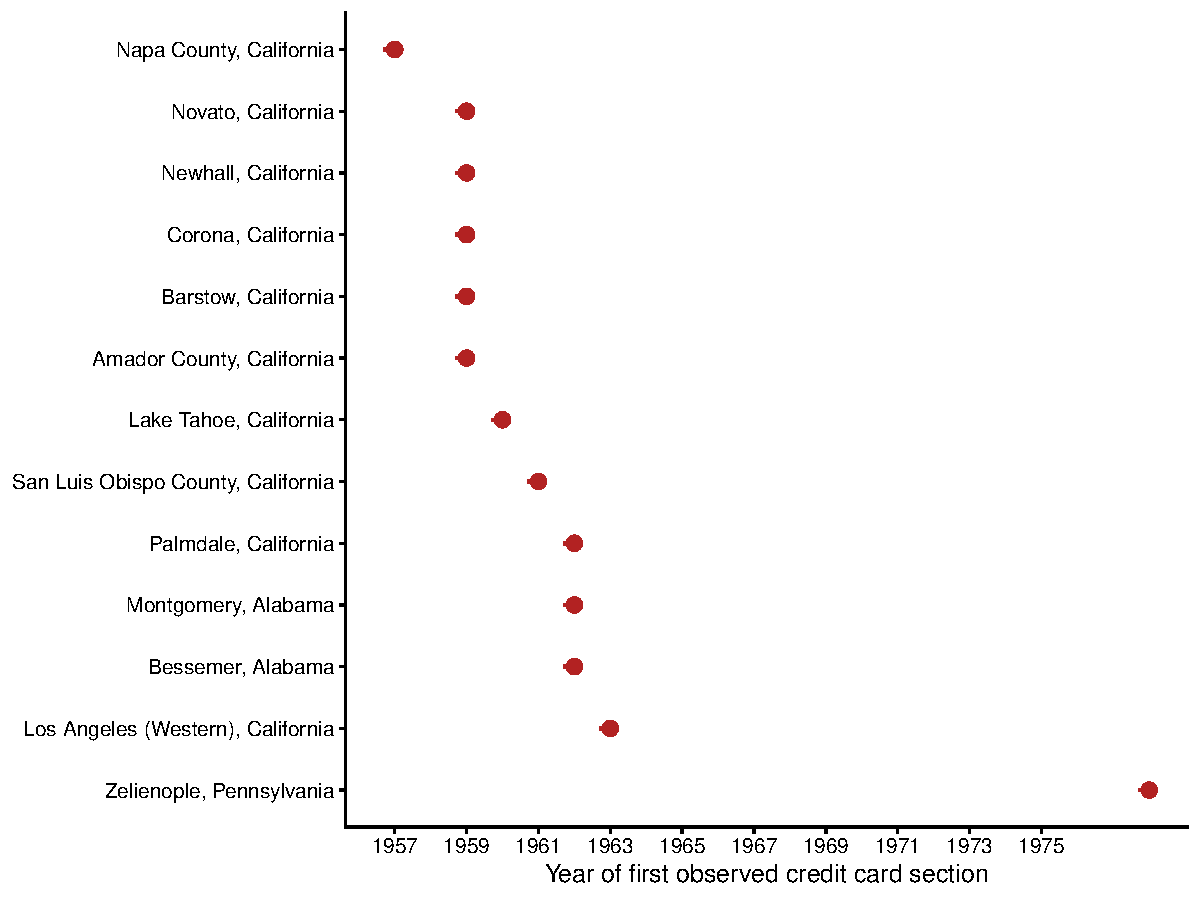
\includegraphics[width=0.85\textwidth]{D_credit_section_intro.pdf}
\end{center}

\textbf{Construction.} For each city where a credit card section was detected in at least one phonebook, I record the earliest year of appearance. Cities are ordered chronologically.

\textbf{Motivation.} This figure shows the diffusion of dedicated ``Credit Card \& Other Credit Plans'' Yellow Pages sections across cities. The earliest appearances cluster around 1967--1970, coinciding with the national expansion of BankAmericard and Master Charge programs. The timeline is informative about the speed and geographic pattern of credit card network penetration into local commercial directories.

%% ============================================================
\newpage
\section*{E. Business Listings by City}

\begin{center}
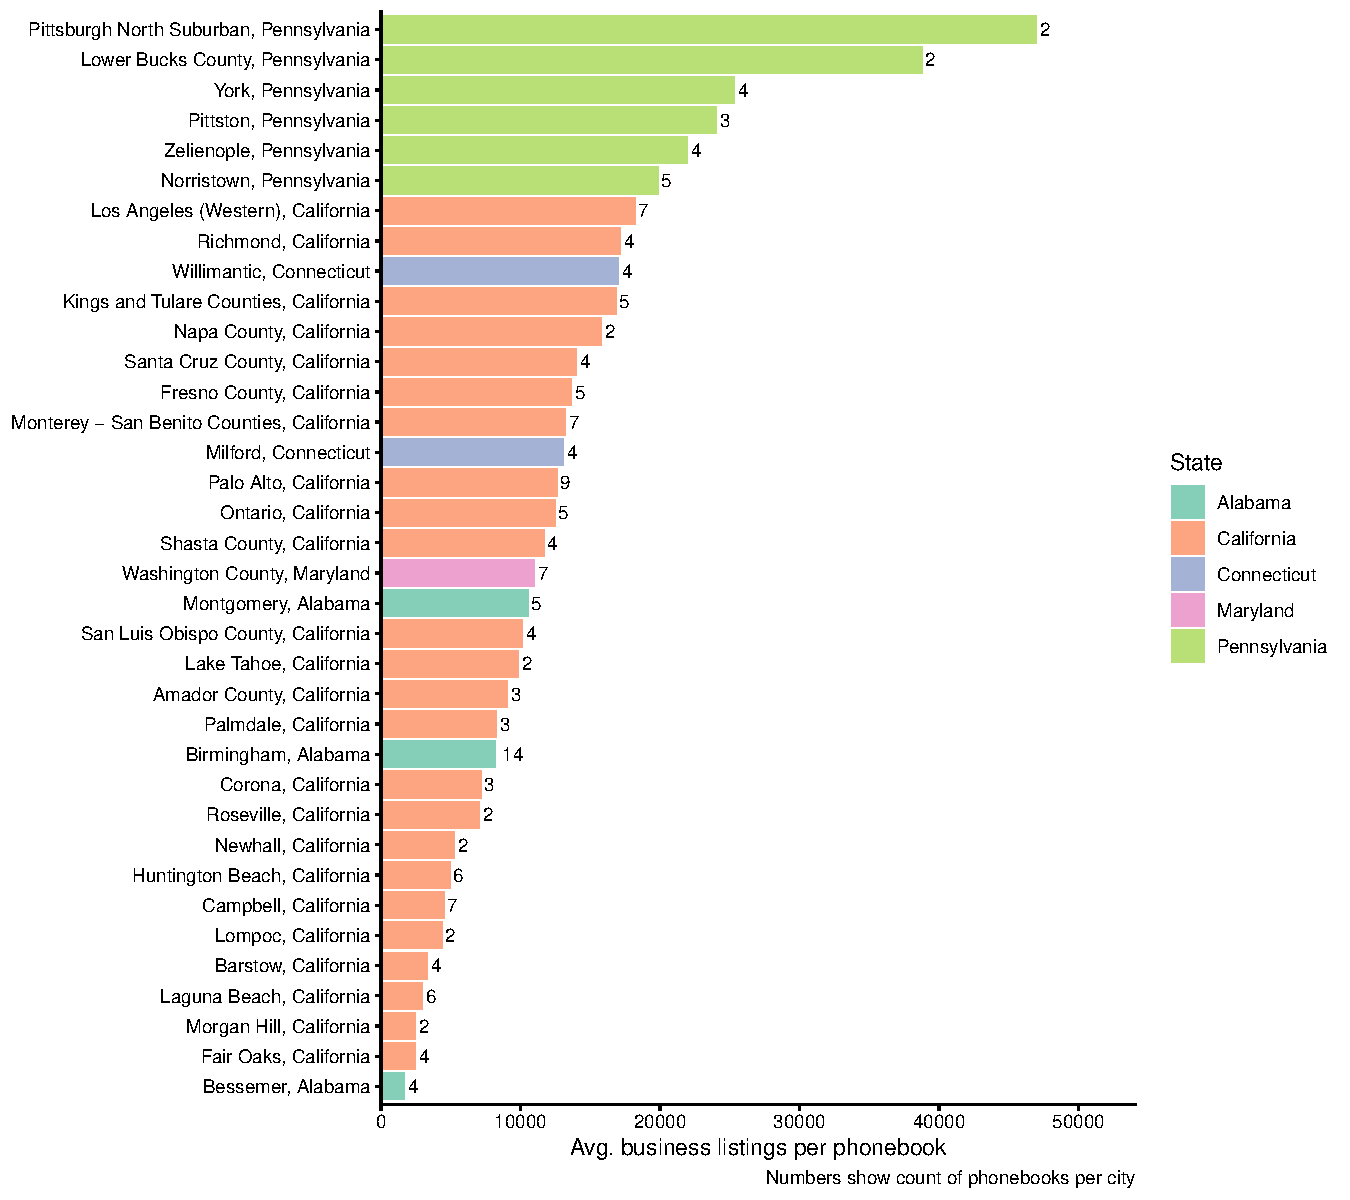
\includegraphics[width=0.85\textwidth]{E_listings_by_city.pdf}
\end{center}

\textbf{Construction.} For cities with at least 2 phonebook-years, I compute the average number of business listings per phonebook. Bar colors indicate state; numbers show the count of phonebooks per city.

\textbf{Motivation.} This figure reveals the variation in market size across the corpus. Large metropolitan areas (Los Angeles, San Francisco, Philadelphia) have an order of magnitude more business listings than small cities (Hagerstown, Pottsville). The listing count proxies for the density of commercial activity and the breadth of the Yellow Pages as a business directory. Cities with more listings are more likely to contain specialized sections, including credit card listings.

%% ============================================================
\newpage
\section*{F. Category Richness Over Time}

\begin{center}
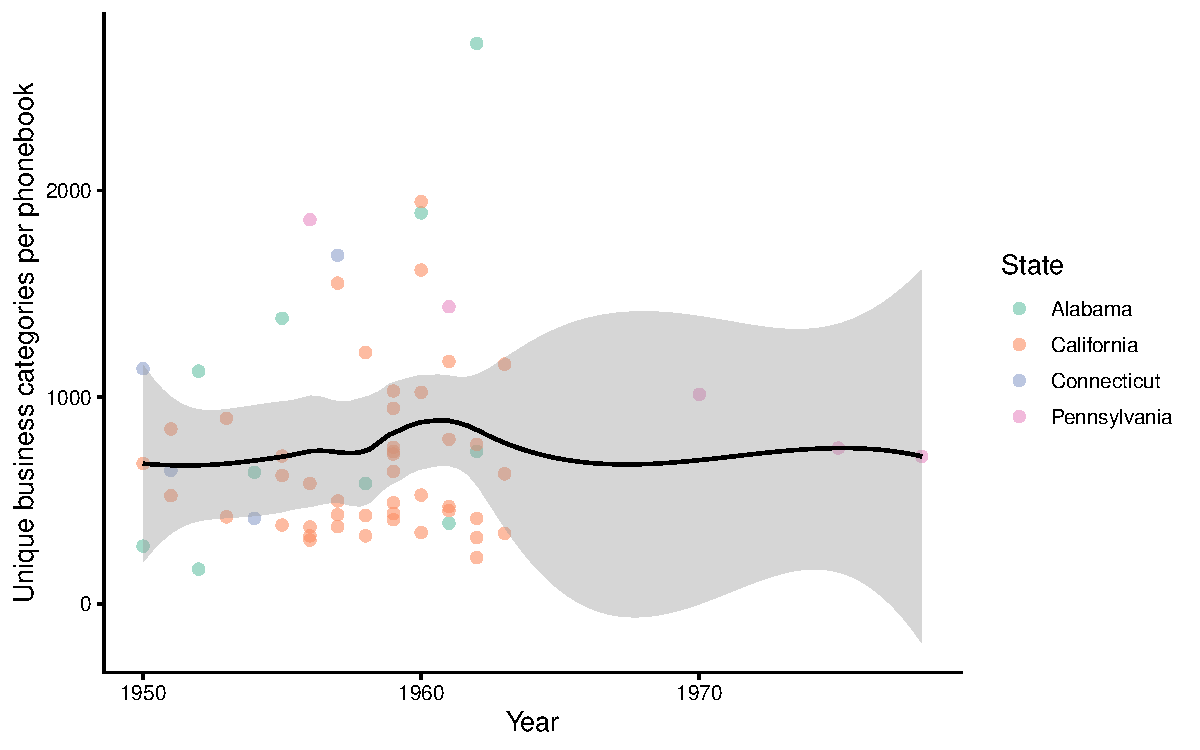
\includegraphics[width=0.85\textwidth]{F_categories_over_time.pdf}
\end{center}

\textbf{Construction.} For each phonebook with category header detection (merged files only), I count the number of unique business categories and plot against year. Points are colored by state; a LOESS smoother shows the trend.

\textbf{Motivation.} The number of distinct Yellow Pages categories reflects the differentiation and specialization of local commercial activity. An upward trend would indicate increasing commercial complexity over the sample period. The variation across states and cities is informative about the heterogeneity of local economies captured by the data. This figure is restricted to merged-file books because page-level-only files lack automated category header detection.

\end{document}
